\chapter[Algoritmo propuesto]{Algoritmo propuesto}
\label{ch:algoritmo}
\section{Pipeline}
\label{sec:pipeline}
Para poder solucionar el problema propuesto en la Sección~\ref{sec:problema}, se propone un algoritmo compuesto por cuatro módulos. \emph{Preprocesamiento de la base de datos}, módulo encargado de quitar todo el ruido de los vídeos de entrenamiento, \emph{extracción de micro-descriptores}, encargado de dividir el vídeo en distintas regiones de interés para crear un micro-descriptor basado en el movimiento interno de éstas, \emph{creación de macro-descriptores}, toma los micro-descriptores y crea un nuevo macro-descriptor por vídeo utilizando técnicas de \textit{clustering}, y por último \emph{entrenamiento y clasificación}, encargado de crear un modelo de clasificación con los descriptores de entrenamiento, para luego utilizar este modelo para la posterior clasificación de nuevos vídeos. Presentamos este modelo en la Figura~\ref{algoritmo:fig:pipeline}.

	\begin{figure}[bt]
		\centering
    		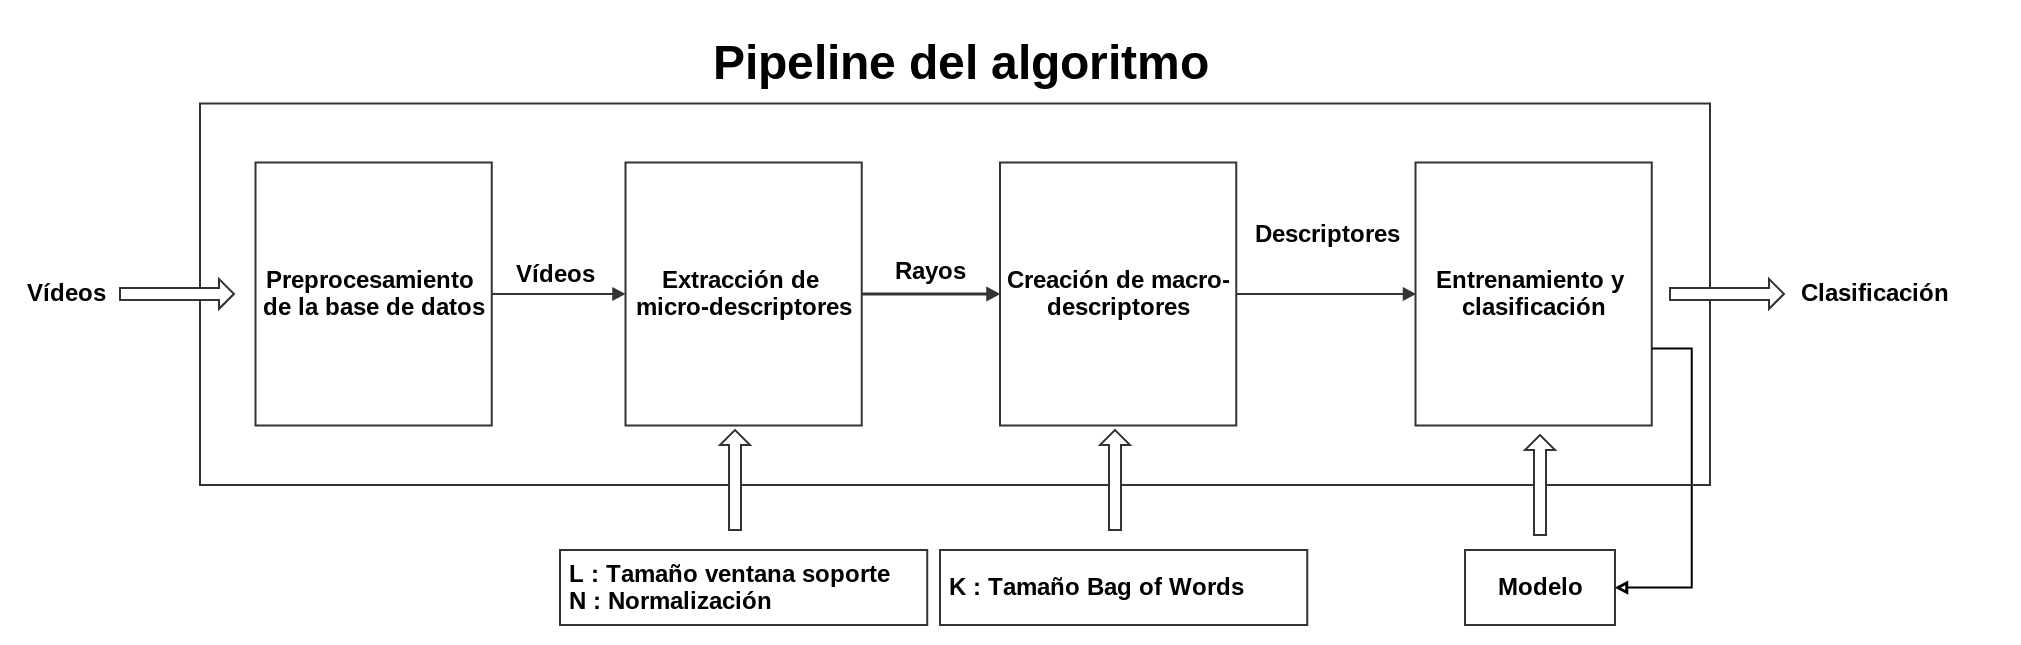
\includegraphics[width=1\textwidth]{Figuras/Diagramas/pipeline.png}
  		\caption{Pipeline del algoritmo propuesto.}
  		\label{algoritmo:fig:pipeline}
	\end{figure}	


\section{Preprocesamiento de la base de datos}
\label{sec:proc_bdd}
%todo corregir este parrafo
	En esta etapa se procede a realizar la limpieza de todos los datos que entran al algoritmo. Cada uno de los vídeos de entrada tienen elementos que no aportan mayor información al método, sino que también pueden aportar ruido, de tal manera se procede a eliminar todos estos elementos. Este procedimiento se divide en dos etapas: \emph{Detección de rostros}, que utiliza el algoritmo de Viola-Jones para encontrar el rostro del primer cuadro, y el segundo \emph{corrección de movimiento}, que utiliza el cuadro encontrado del rostro para corregir el movimiento de todos los cuadros del vídeo. Este procedimiento puede ser visualizado en la Figura~\ref{algoritmo:fig:preprocesamiento}. 
	
	\begin{figure}[tb]
		\centering
    		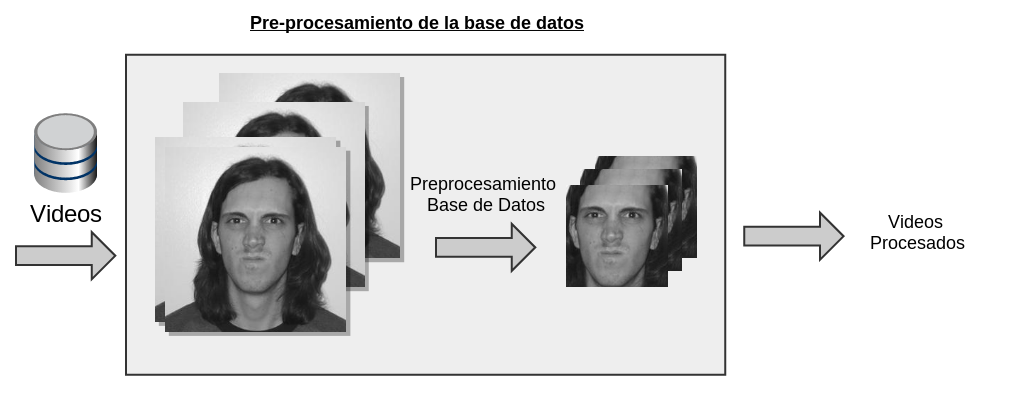
\includegraphics[width=1\textwidth]{Figuras/Diagramas/Preprocesamiento.png}
  		\caption{Diagrama del preprocesamiento de los datos.}
  		\label{algoritmo:fig:preprocesamiento}
	\end{figure}	

	
	\subsection{Detección de rostros}
	\label{algoritmo:det_rostro}
	Para cada uno de los vídeos que se utilizarán en el algoritmo es necesario quitar todos los elementos que no aportan información. De tal forma, utilizamos un algoritmo de detección de rostros, el cual obtiene los vértices del rectángulo que encierra la cara en el primer cuadro. Utilizaremos este rectángulo en la fase de corrección de movimiento del rostro. 
		
	\subsection{Corrección de movimiento}
	\label{algoritmo:cor_movimiento}
	Luego de realizar la detección de rostros para cada uno de los cuadros del vídeo, se procede a realizar la corrección del movimiento rígida. Ésta consiste en realizar operaciones de translación y rotación sobre cada uno de los cuadros del vídeo utilizando la imagen del rostro detectado en el primer cuadro como modelo para ajustar los cuadros siguientes.


\section{Extracción de micro-descriptores}
\label{sec:micro_descriptores}
	El proceso de extracción de micro-descriptores es el núcleo del algoritmo. Este proceso es el encargado de la extracción de características directas del vídeo o imagen dinámica. Para esto se introduce un nuevo término que es denominado \textit{Rayo de flujo} o simplemente \textit{Rayo}. Éste define el movimiento de los píxeles dentro las regiones de interés (ROI por sus siglas en inglés) en los cuadros del vídeo. Esta etapa se puede dividir en tres grandes bloques, primero, la \emph{codificación}, etapa en la cual el vídeo puede ser codificado utilizando técnicas como LBP o LDN\@. Esta etapa es opcional y sera mayormente profundizada en el Capít ulo~\ref{ch:exp_result}. Segundo, \emph{extracción de rayos}, la cual consiste en determinar las regiones de interés de donde se extraerán los \textit{Rayos de flujo}, y su extracción como tal. Y por ultimo, \emph{normalización}, esta etapa se encarga de llevar todos los \textit{Rayos} al mismo espacio vectorial, dado un tamaño fijo. Un diagrama de la extracción de micro-descriptores puede ser visto en la Figura~\ref{algoritmo:fig:micro_descriptores}.

\afterpage{% corrige el breakpage
\begin{landscape}
	\begin{figure}[t]
		\centering
    		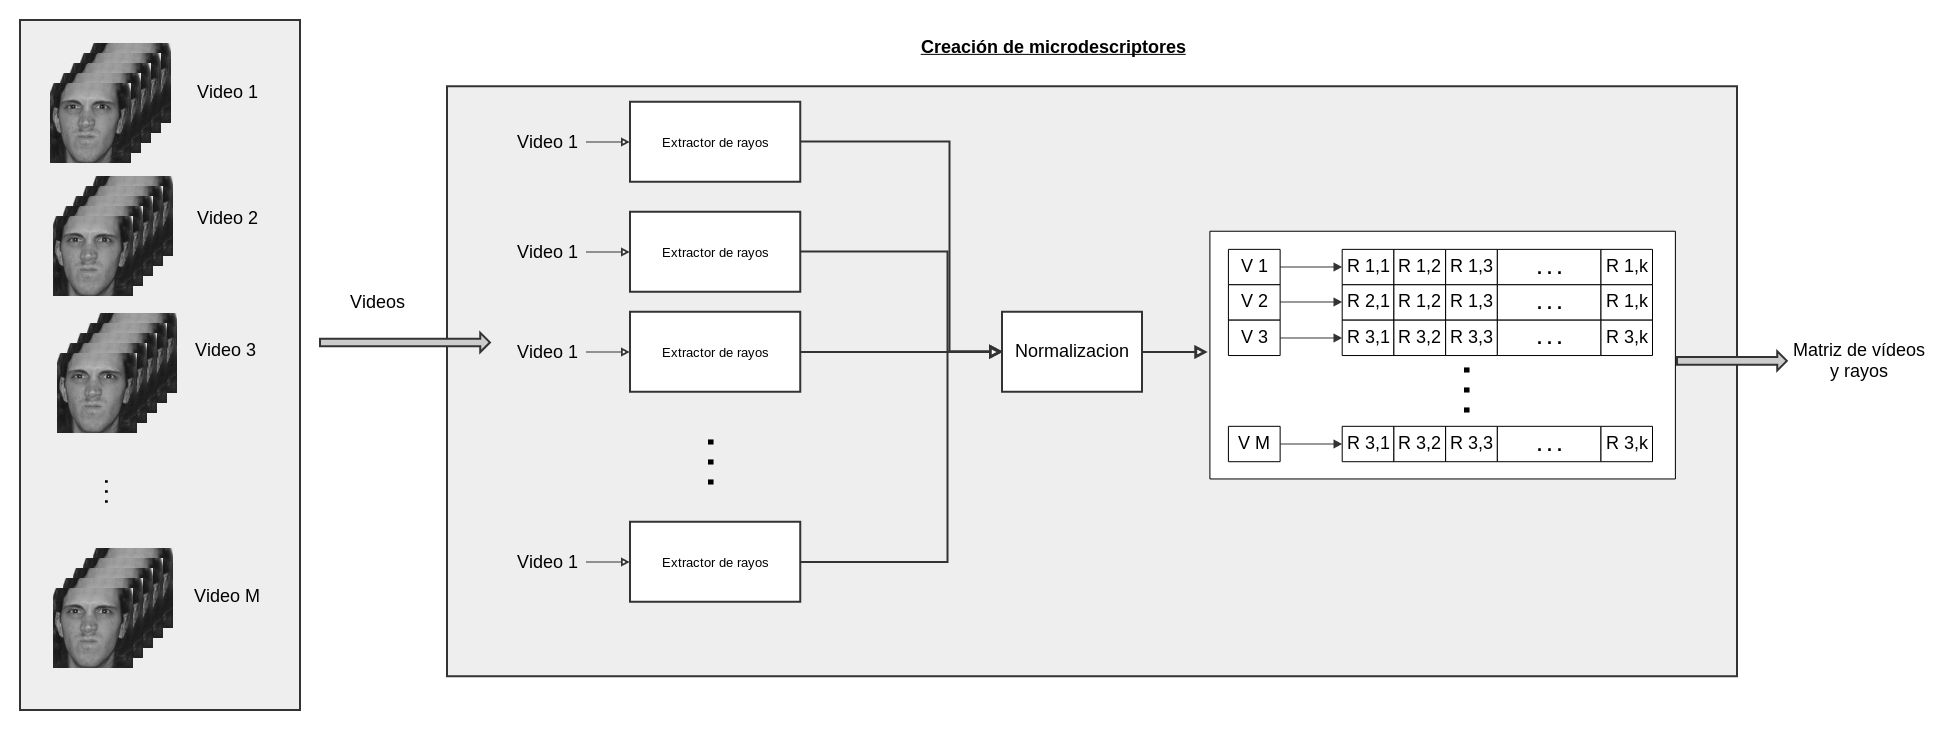
\includegraphics[width=\linewidth]{Figuras/Diagramas/Extractor_microdescriptores}
  		\caption{Diagrama general del proceso de extracción de micro-des\-crip\-to\-res.}
  		\label{algoritmo:fig:micro_descriptores}
	\end{figure}	
\end{landscape}}

	\subsection{Elección de regiones de interés}
	\label{algoritmo:elecc_roi}
	De cada vídeos que se quiere procesar, después de realizar el preprocesamiento definido en la Sección~\ref{sec:proc_bdd}, se seleccionan las regiones de interés a las cuales se les extraerá los \textit{Rayos}. Las áreas se seleccionarán utilizando distintos criterios [$\mathds{R}(\cdot)$, ver (\ref{algoritmo:eq:roi})], por ejemplo, pueden utilizarse áreas puntuales con alta expresividad (\eg, los ojos, la boca, la nariz, \etc), o bien áreas generales (\eg, todo el rostro).
	
	De tal forma, definimos un vídeo como 
	\begin{equation}\label{algoritmo:eq:video}		
		V = \{\text{ROI}_i | 1 \leq i \le I\}, 
	\end{equation}
	donde $I$ es el número de regiones de interés en el vídeo. Y además, definimos el $i$-ésimo ROI, $\text{ROI}_i^t$, como el conjunto de píxeles $(x,y)$ para un determinado cuadro $t$, tal que
	\begin{equation}\label{algoritmo:eq:roi}
		\text{ROI}_{i}^{t} = \{(x,y) | (x,y,t) \in \mathds{R}(i)\},
	\end{equation}
	donde $\mathds{R}(i)$, es una función que devuelve la $i$-ésima región en que dividimos el vídeo, según el criterio antes mencionado.

	\subsection{Extracción de rayos}
	\label{algoritmo:ext_rayos}
	
	Para esta sección se introducen dos términos nuevos: la \textit{región de soporte} y la \textit{ventana de búsqueda}. La \textit{región de soporte} es utilizada para calcular el movimiento del píxel central con respecto al cuadro siguiente. Similarmente, la \textit{ventana de búsqueda} es el espacio supuesto en el cual se puede haber desplazado la región de soporte en el siguiente cuadro, y por ende, donde lo buscaremos. Definimos estos términos formalmente a continuación.
	
	\begin{definition}[Región de soporte]	
  Dado un píxel $(x,y)$ en un cuadro $t$, definimos una región de soporte RS, de tamaño $L \times L$ (donde $L$ es impar), como la subregión del cuadro $t$ que está centrada en el píxel $(x,y)$.
	\end{definition}

	\begin{definition}[Ventana de búsqueda]
	Dado un píxel $(x,y)$ en un cuadro $t$, definimos la ventana de búsqueda WS, de  tamaño $(2L+1) \times (2L+1)$, como la subregión del cuadro $t+1$ que está centrada en el píxel $(x,y)$.
	\end{definition}
		
	Dado un píxel $(x,y)$ en el cuadro $t$, la extracción de rayos consiste en obtener una \textit{región de soporte}, $\text{RS}(x,y,t)$, una \textit{ventana de búsqueda}, $\text{WS}(x,y,t)$, y encontrar la posición de mejor emparejamiento entre la \textit{región de soporte} y la \textit{ventana de búsqueda}. Esta búsqueda se realiza calculando el error Cuadrático Medio (MSE por sus siglas en inglés), \begin{equation}\label{algoritmo:eq:mse}	
			\text{MSE}(\text{RS}, \text{RS}') = \sum_{x=1}^{L} \sum_{y=1}^{L} (\text{RS}(x,y,t) - \text{RS}'(x',y', t+1))^2,
		\end{equation} 
	donde $\text{RS} = \text{RS}(x,y,t)$ es la \textit{región de soporte} del píxel $(x,y)$ en el cuadro $t$, al que esta extrayendo el \textit{rayo}, y $\text{RS}' = \text{RS}'(x',y',t+1) \in \text{WS}(x,y,t)$ es una subregión de la \textit{ventana de búsqueda} del píxel $(x,y)$ en el cuadro $t+1$ de tamaño $L$ (note que la \textit{ventana de búsqueda} del píxel $(x,y)$ en el cuadro $t$ está definida en el cuadro $t+1$).
		
	Esta operación se realiza para cada uno de los desplazamientos que puedan ser realizados por la \textit{región de soporte} dentro de la \textit{ventana de búsqueda}. De tal forma que buscamos la posición de la región $\text{RS}'$ que minimiza el MSE respecto de la \textit{región de soporte} del píxel $(x,y)$ en el cuadro $t$, $\text{RS}(x,y,t)$, de tal forma que la región $\text{RS}'$ óptima será
	\begin{equation}
		\text{RS}^* = \arg \min_{\text{RS}'}\{\text{MSE}(\text{RS},\text{RS}') | \text{RS}' \in \text{WS} \},
	\end{equation}		
	la cual será la posición donde la \textit{región de soporte} se desplazó en el cuadro $t+1$. Con esto se obtiene el píxel $(x^*,y^*)$ que corresponde al centro de la ventana obtenida en el proceso anterior, $\text{RS}^*$.
	
	Para calcular el desplazamiento en el cuadro $t$ de $(x,y)$ a $(x^*,y^*)$, se procede a realizar la resta de los ejes. De tal forma que
	\begin{align}
		\Delta x^{t} &= x-x^*,\\ 
		\Delta y^{t} &= y-y^*.
	\end{align}
		Donde $ \Delta x^*$ y $ \Delta y^*$ son componentes del \textit{Rayo de soporte}, definimos un \textit{Rayo de soporte} como
	\begin{equation}
		\rho_{(x,y)} = \{(\Delta x^{t}, \Delta y^{t})~| \forall t\}.
	\end{equation}		
	Los \textit{Rayos de soporte} son la estructura básica de los \textit{Rayos de flujo}, dado que al juntar todos los desplazamientos del píxel $(x,y)$ a lo largo de los cuadros del vídeo, se obtiene un conjunto de variaciones de movimientos de estos. Este conjunto es definido como \textit{rayo de flujo} o micro-descriptor,
	\begin{equation}
		R(x,y)	 = \{\rho_1(x,y), \rho_2(x^*,y^*), \rho_3(x^{**},y^{**}), ... \},
	\end{equation}
	donde ($x^{**}$,$y^{**}$) es el píxel al cual se desplazo ($x^{*}$,$y^{*}$) en el cuadro $t+2$. El desplazamiento de los \textit{rayos} puede ser visto en la Figura~\ref{algoritmo:fig:normalizacion}.
		
		%%HABLAR DE ventana de soporte, ventana de busqueda MSE
		
	\subsection{Normalización de rayos}
	\label{algoritmo:normalizacion}
	Luego de obtener el total de micro-descriptores es necesario poder llevar todos los \textit{rayos} al mismo espacio vectorial, esto debido a que el tamaño de cada conjunto depende de la cantidad de cuadros $T$ del vídeo. Para este proceso se introduce una variable muy importante para el algoritmo llamada $N$, esta sera la encargada de comandar el proceso de normalización, de tal forma que se obtiene una razón de normalización
	\begin{equation}
		Rn = \frac{T}{N},
	\end{equation}
	está permite relacionar la cantidad de \textit{Rayos de soporte} $\rho$ del \textit{Rayo} $R(x,y)$ original que formaran parte de los $\rho'$ de $R(x,y)'$ normalizado. Este proceso puede ser visualizado en la Figura~\ref{algoritmo:fig:normalizacion}.
	
	\begin{figure}[bt]
		\centering
    		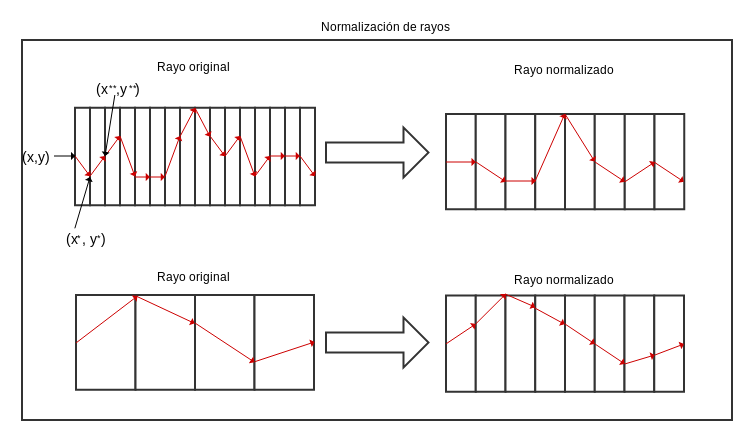
\includegraphics[width=1\textwidth]{Figuras/Diagramas/normalizacion_de_rayos.png}
  		\caption{Representación y Normalización de rayos.}
  		\label{algoritmo:fig:normalizacion}
	\end{figure}	

	
\newpage	
\section{Creación de macro-descriptores}
\label{sec:macro-descriptores}
El proceso de creación de macro-descriptores es el proceso final de la extracción de características de los vídeos. Luego de obtener un extenso conjunto de \textit{Rayos} para cada uno de los vídeos, es necesario poder crear grupos de \textit{Rayos}, los cuales puedan representar de mejor manera el espacio ya normalizado. Para esto se utilizan técnicas de \textit{clustering}. El proceso de Creación de macro-descriptores puede ser visto en las Figuras~\ref{algoritmo:fig:macro_descriptores:entrenamiento} y~\ref{algoritmo:fig:macro_descriptores:clasificacion}

	\begin{figure}[bt]
		\centering
    		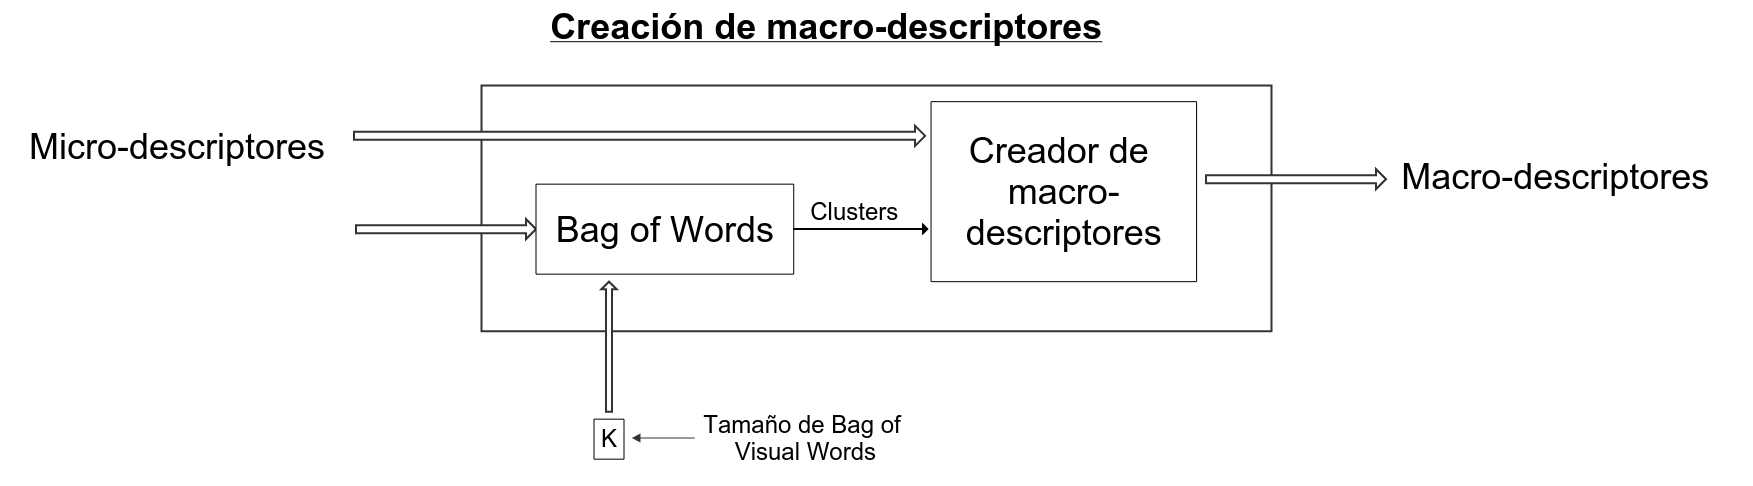
\includegraphics[width=1\textwidth]{Figuras/Diagramas/Extractor_macrodescriptores_entrenamiento.png}
  		\caption{Proceso de creación de macro-descriptores en la fase de entrenamiento.}
  		\label{algoritmo:fig:macro_descriptores:entrenamiento}
	\end{figure}	
	
	
	\begin{figure}[bt]
		\centering
    		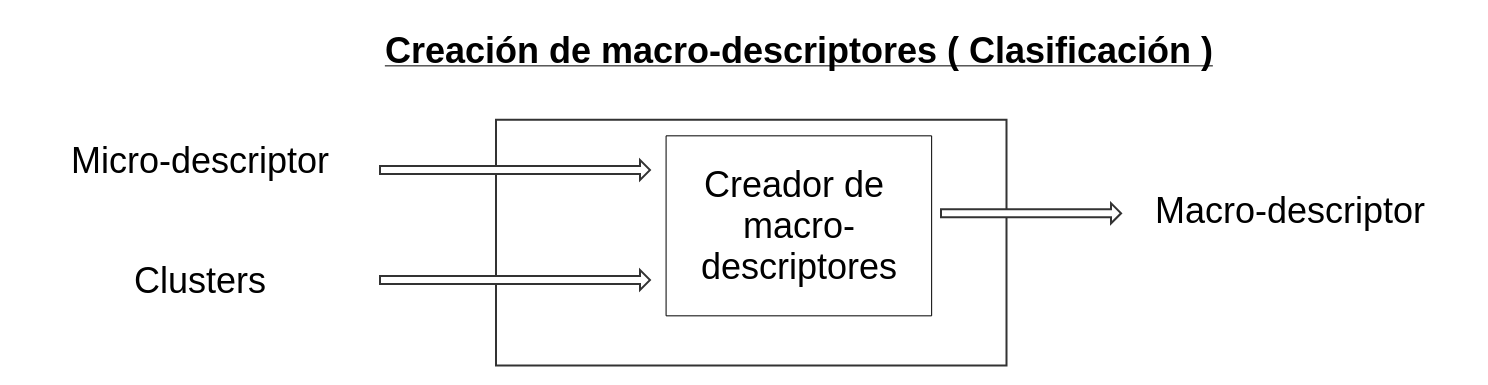
\includegraphics[width=1\textwidth]{Figuras/Diagramas/Extractor_macrodescriptores_clasificacion.png}
  		\caption{Proceso de creación de macro-descriptores en la fase de clasificación.}
  		\label{algoritmo:fig:macro_descriptores:clasificacion}
	\end{figure}	



	\subsection{Bag of Visual Words}
	\label{algoritmo:bow}
		Esta es una técnica dependiente de la cantidad $K$ de palabras que se introduzcan a la bolsa. Como se puede observar en la Figura~\ref{algoritmo:fig:bow}, esta técnica permite armar $K$ grupos representados por un centroide o \textit{cluster} llamado $C_k$. Estos \textit{clusters} son los puntos de referencia de cada uno de estos grupos. Para saber a cual de los $K$ centroides pertenece un \textit{Rayo} $R(x,y)$, es necesario calcular el
		\begin{equation}
  			\label{algoritmo:eq:dist}
			k^* = \arg \min_k \{\mathit{dist}(R(x,y),C_k)\},
		\end{equation}
		donde la función de distancia $\mathit{dist}(\cdot,\cdot)$ depende del experimento que se este realizando, las métricas de distancia a utilizar pueden ser vistas en la Sección~\ref{sec:matricas_de_distancia}.

	\begin{figure}[tb]
		\centering
    		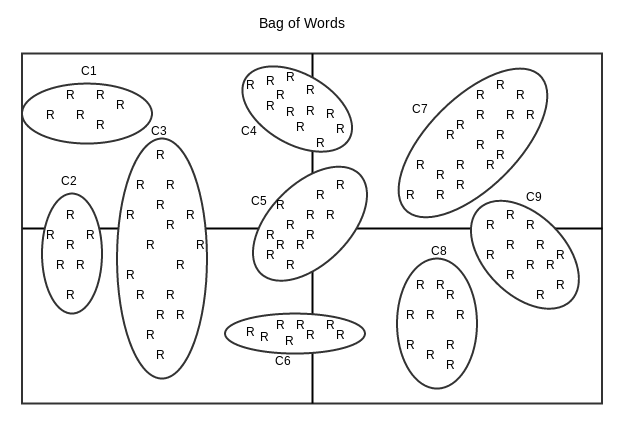
\includegraphics[width=1\textwidth]{Figuras/Diagramas/bow_solo.png}
  		\caption{Construcción del Bag of Words.}
  		\label{algoritmo:fig:bow}
	\end{figure}	

	\subsection{Creación de macro-descriptores}
	\label{algoritmo:crea_macro-descriptores}
	Luego de tener etiquetado cada uno de los \textit{Rayos} $R(x,y)$ con su centroide respectivo, se procede a crear el macro-descriptor de cada uno de los vídeos.	 Esto se realiza creando un histograma de tamaño $K$ para cada uno de las regiones de interés ${ROI}_{i}^{t}$ del vídeo, de tal forma que en este histograma se tenga presente la frecuencia de cada uno de los \textit{clusters} encontrados en la creación del \textit{Bag of Visual Words}. Con esto presente, definimos el descriptor $D_i$ de la región de interés $\text{ROI}_i$ como
	\begin{align}
		\label{algoritmo:eq:hist}
		D_i(k) &= \sum_{(x,y)\in \text{ROI}_i} \delta (R(x,y),k) \quad \forall k\\
		\label{algoritmo:eq:fun_hist}
		 \delta (R(x,y),k) &= \begin{cases}
		 1 & \mbox{si }R(x,y)~\in~C_k\\
     0 & \text{otro caso}
     \end{cases},
	\end{align}
de tal forma que $\delta(\cdot,\cdot)$ es una función que cuenta los rayos pertenecientes al \textit{cluster} $k$, $C_k$.
%		 \left \{ \begin{matrix} 1 & \mbox{si }R(x,y)\mbox{ \in C_k} \\ 0 & \mbox{}\mbox{de otra forma}\end{matrix}\right. 		


	
	Luego de obtener dichos descriptores por región, se procede a concatenar cada uno de los histogramas pertenecientes al mismo vídeo de la siguiente forma
	\begin{equation}
		\mathds{D} = \cat_{i = 1}^{I} D_i, \quad \forall i,
	\end{equation}	   
   donde $\cat$ es el operador de concatenación de los vectores $D_i$. Este proceso puede ser visto en la Figura~\ref{algoritmo:fig:macrodescriptores}. El resultado de esta concatenación es el macro-descriptor del vídeo seleccionado.
   
   	\begin{figure}[bt]
		\centering
  		\label{algoritmo:fig:macrodescriptores}
    		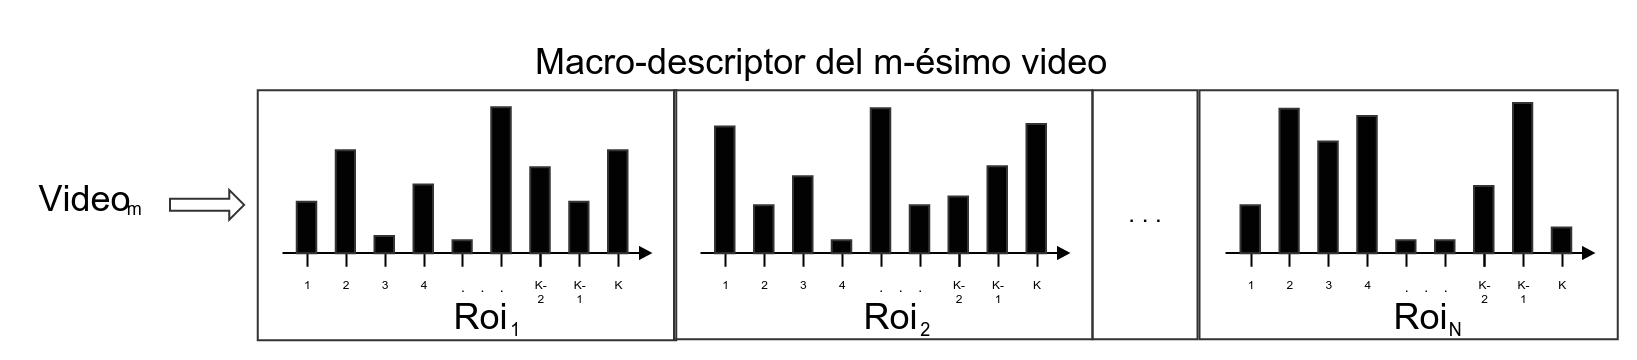
\includegraphics[width=1\textwidth]{Figuras/Diagramas/macro-descriptor.png}
  		\caption{Construcción del macro-descriptor.}
	\end{figure}	


	En el proceso clasificación, no se recalculan los centroides para un nuevo vídeo, ya que, se guarda el modelo que contiene el resultado del \textit{Bag of Visual Words}, y se procede a calcular~(\ref{algoritmo:eq:dist}), para cada uno de los \textit{Rayos} $R(x,y)$ obtenidos en el proceso de extracción de micro-descriptores. Luego de esto al igual que en el proceso de entrenamiento se crea el macro-descriptor con el mismo método.
	
	
\section{Entrenamiento y clasificación}
\label{sec:clasificacion}
Ultima etapa del algoritmo, se dedicada a la segmentación del espacio vectorial formado por los macro-descriptores. Para este proceso se utilizara las \textit{Support Vector Machines}, explicadas en la Sección~\ref{sec:rec_patrones}. Estás se utilizan para entrenar el modelo que luego es utilizado para clasificar las nuevas entradas de vídeo. 
Para poder probar la efectividad del clasificador se utilizaran técnicas de validación cruzada o $k$\textit{-fold cross-validation} (Por sus siglas en inglés). Esta técnica consiste en dividir el conjunto de datos de datos en dos grupos, uno de entrenamiento y uno de prueba, $k$ veces. Esta técnica es utilizada para correr el algoritmo en distintas instancias, y así poder obtener un valor mas real de la precisión. Se mostraran los resultados de esta técnica en la Capítulo~\ref{ch:exp_result}.


	\subsection{Entrenamiento}
	\label{algoritmo:entrenamiento}
		Luego de que el conjunto de datos de entrenamiento pasa por todas las etapas anteriores del algoritmo, se tiene para cada uno de los vídeos un macro-descriptor compuesto por la concatenación de los histogramas de de cada una de las regiones de interés y una etiqueta que indica a que clase pertenecen. Este conjunto de descriptores y las etiquetas son utilizados por las \textit{Support Vector Machines} para la creación de un modelo de clasificación, el que permite poder etiquetar nuevas entradas, este proceso puede ser visto en la Figura~\ref{algoritmo:fig:entrenamiento}.
	
	Las \textit{Support Vector Machines}, al ser un clasificador de dos clases, es necesario utilizar técnicas que permita realizar la clasificación utilizando muchas clases, para el caso de esta implementación es necesario poder generar un modelo que permita clasificar las seis expresiones universales. Con este motivo se utiliza la técnica \textit{Uno contra uno}, la cual consiste en generar $\frac{C(C-1)}{2}$ clasificadores, donde cada clase tiene una barrera de decisión asociada a cada una de las demás clases. Esto permite que la región de incertidumbre formada por las barreras de decisión sea mínima.
		
		
	\begin{figure}[bt]
		\centering
  		\label{algoritmo:fig:entrenamiento}
    		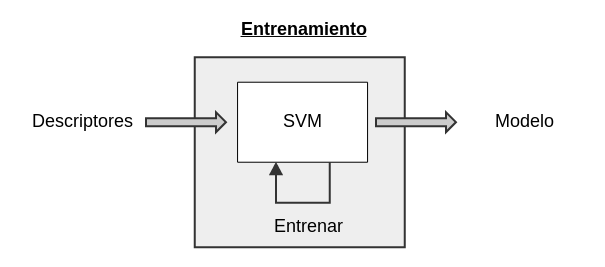
\includegraphics[width=0.7\textwidth]{Figuras/Diagramas/Entrenamiento.png}
  		\caption{Entrenamiento del clasificador.}
	\end{figure}	
		
		
	\subsection{Clasificación}
	\label{algoritmo:clasificacion}
		Ya teniendo el modelo resultante de la etapa de entrenamiento, esté es utilizado para la clasificación de nuevas entradas sin etiquetar, esto con la misión de poder asignar una etiqueta al nuevo descriptor, este proceso puede ser visto en la Figura~\ref{algoritmo:fig:clasificacion}. En esta etapa se puede medir cual es la precision del algoritmo, esta medición sera mayormente abordada en el Capítulo~\ref{ch:exp_result}.
		
	
	\begin{figure}[bt]
		\centering
  		\label{algoritmo:fig:clasificacion}
    		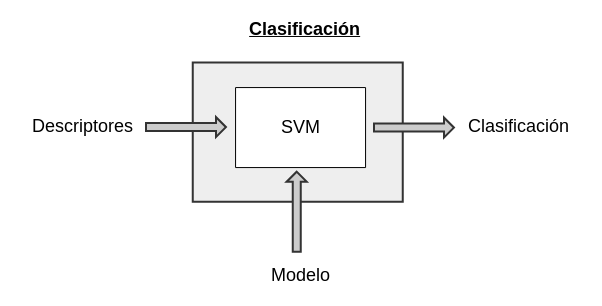
\includegraphics[width=0.7\textwidth]{Figuras/Diagramas/Clasificacion.png}
  		\caption{Clasificador utilizando el modelo creado para clasificar nuevas entradas.}
	\end{figure}	
		
	
	
	
	
	